\documentclass[11pt,twocolumn]{article}

% ── Packages ──────────────────────────────────────────────
\usepackage[margin=0.75in]{geometry}
\usepackage{booktabs}
\usepackage{graphicx}
\usepackage{hyperref}
\usepackage{listings}
\usepackage{xcolor}
\usepackage{float}
\usepackage{caption}
\usepackage{subcaption}
\usepackage{amsmath}
\usepackage{enumitem}
\usepackage{url}
\usepackage{multirow}
\usepackage{array}
\usepackage{adjustbox}
\usepackage[numbers]{natbib}
\usepackage{dblfloatfix} % fix float placement in twocolumn
\usepackage{tikz}
\usetikzlibrary{positioning,arrows.meta,calc}

\lstset{
  basicstyle=\ttfamily\scriptsize,
  breaklines=true,
  frame=single,
  backgroundcolor=\color{gray!8},
  keywordstyle=\color{blue!70},
  commentstyle=\color{green!50!black},
  stringstyle=\color{red!60},
  showstringspaces=false,
}

\hypersetup{
  colorlinks=true,
  linkcolor=blue!60!black,
  citecolor=blue!60!black,
  urlcolor=blue!60!black,
}

% ── Convenience ───────────────────────────────────────────
\graphicspath{{../../charts/}}

% ── Title ─────────────────────────────────────────────────
\title{\textbf{OSS Pulse: How Coding Agents Reshaped\\Open-Source Development}\\[6pt]
\large Tracking 1.46 Billion GitHub Events Across the 2022--2026 Agent Era}

\author{
  Jhe Chen Li (jl17797) \qquad Bo Yu (by2566)\\
  \textit{Group 9 --- BDAD Spring 2026, New York University}
}

\date{May 2026}

\begin{document}
\maketitle

% ══════════════════════════════════════════════════════════
\begin{abstract}
We present \textbf{OSS Pulse}, a large-scale empirical study of open-source software ecosystem health across the 2022--2026 coding agent era.
By combining 1.46~billion GitHub Archive events (five quarterly snapshots), 2.8~million Hugging Face Hub model records, and PyPI download statistics for 46 AI/ML libraries, we construct a multi-dimensional health framework that goes beyond traditional star-based metrics.
Our analysis reveals three structural shifts: (1)~development became \emph{lighter}---51\% more developers but 42\% fewer contributors per repository; (2)~the weekend activity gap closed---weekend share rose from 25.8\% to 29.7\%, consistent with (though not proof of) round-the-clock automation; and (3)~high-frequency push activity exhibited a two-phase pattern---explosive growth in 2025 followed by normalization in 2026, plausibly tracking but not equivalent to coding-agent adoption.
We processed 930+~GB of raw data into 87.9~GB of cleaned Parquet files through 10 Spark analytics jobs on a Google Cloud Dataproc cluster.
\end{abstract}

% ══════════════════════════════════════════════════════════
\section{Introduction}\label{sec:intro}

GitHub stars have long served as a proxy for open-source project health.
However, in the era of coding agents---tools such as Cursor~\cite{cursor}, Claude Code~\cite{claudecode}, and Devin~\cite{devin} that automate large portions of the software development workflow---this proxy is breaking down.
DeepSeek-R1, for instance, is among GitHub's most-starred repositories with over 93,000 watchers, yet only 5 distinct accounts pushed code to it during 2026-Q1.

The period from 2022 to 2026 spans a remarkable transformation in software development: from the pre-ChatGPT baseline (2022), through the LLM explosion (2023--2024), into the agent era (2025--2026).
We hypothesize that coding agents are fundamentally altering open-source contribution patterns, and that traditional metrics fail to capture these changes.

\textbf{Research questions.}
\begin{enumerate}[nosep]
  \item How has the macro-level structure of the OSS ecosystem changed across five annual snapshots?
  \item Do coding agents produce measurable changes in development rhythms?
  \item Can a multi-dimensional health score better characterize project vitality than star counts alone?
\end{enumerate}

\textbf{Contributions.}
\begin{itemize}[nosep]
  \item A longitudinal dataset of 1.46B GitHub events across five Q1 snapshots (2022--2026).
  \item A composite health score integrating Hugging Face adoption, PyPI downloads, and GitHub activity.
  \item Empirical evidence of three structural shifts in OSS development driven by coding agents.
  \item An open-source Spark pipeline of 10 analytics jobs.
\end{itemize}

% ══════════════════════════════════════════════════════════
\section{Related Work}\label{sec:related}

\textbf{OSS health metrics.}
Coelho and Valente~\cite{coelho2017} characterized failure modes of modern OSS projects through commit and contributor decay; Avelino et al.~\cite{avelino2016} formalized the \emph{truck factor} as a commit-based concentration measure.
We extend the same intuition from commits to PR-level diversity, and complement it with cross-platform demand signals (Hugging Face, PyPI).
The CHAOSS project~\cite{chaoss} maintains a catalogue of standardized community-health indicators, but most published indicator studies predate the agent era.

\textbf{GitHub star inflation.}
He et al.~\cite{he2024fakestars} identified approximately 6~million suspected fake stars on GitHub between 2019 and 2024, with a substantial fraction of the flagged repositories subsequently removed.
Our 2026-Q1 observation---a 63\% year-over-year drop in WatchEvents---is \emph{consistent with} the tail of this clean-up, although the magnitude of the drop suggests additional factors (\S\ref{sec:findings}).

\textbf{AI-assisted development.}
Recent surveys document the rise of LLM-driven coding tools and agents~\cite{fan2023}, but empirical, ecosystem-wide quantitative analyses of their behavioral fingerprint on public-repository activity remain scarce.
Our work fills this gap by quantifying behavioral shifts across 1.46B events.

% ══════════════════════════════════════════════════════════
\section{Data Sources}\label{sec:data}

We integrate three complementary data sources to enable multi-dimensional health assessment.

\subsection{GitHub Archive}

GH Archive\footnote{\url{https://www.gharchive.org/}} provides hourly snapshots of all public GitHub events.
We collected five Q1 windows (January--March) for 2022 through 2026, plus the full 2025 calendar year as supplementary data.
Table~\ref{tab:data-scale} summarizes the scale.
Five event types are retained: \texttt{PushEvent}, \texttt{PullRequestEvent}, \texttt{WatchEvent}, \texttt{IssuesEvent}, and \texttt{ForkEvent}.

\begin{table}[t]
\centering\small
\caption{GitHub Archive data scale per era.}\label{tab:data-scale}
\begin{tabular}{@{}lrrr@{}}
\toprule
\textbf{Era} & \textbf{Events} & \textbf{Repos} & \textbf{Actors} \\
\midrule
2022-Q1 & 206.8M & 17.0M & 7.0M \\
2023-Q1 & 247.4M & 19.9M & 7.8M \\
2024-Q1 & 364.4M & 17.6M & 8.9M \\
2025-Q1 & 376.4M & 20.2M & 10.2M \\
2026-Q1 & 265.9M & 20.9M & 10.6M \\
\midrule
\textbf{Total} & \textbf{1.46B} & --- & --- \\
\bottomrule
\end{tabular}
\end{table}

\subsection{Hugging Face Hub}

We captured a snapshot of the Hugging Face Hub in April 2026, comprising 2,815,064 model records.
Key fields include \texttt{modelId}, \texttt{pipeline\_tag}, \texttt{library\_name}, \texttt{downloads} (30-day), \texttt{likes}, and \texttt{parameter\_count}.
The data was ingested via the \texttt{huggingface\_hub} Python API and processed through the same PySpark pipeline used for GH Archive.

\subsection{PyPI Download Statistics}

Monthly download counts for 46 AI/ML Python libraries were obtained via Google BigQuery's public PyPI dataset, covering all 12 months of 2025.

\subsection{Seed Repository List}

We curated 93 AI/ML repositories spanning 14 categories (frameworks, LLM serving, inference, agents, RAG, diffusion, training, evaluation, etc.) to enable focused AI-vs-general comparisons.

% ══════════════════════════════════════════════════════════
\section{Pipeline Architecture}\label{sec:pipeline}

\subsection{System Overview}

The pipeline runs on NYU's Google Cloud Dataproc cluster.
All data is stored in HDFS as Parquet files partitioned by \texttt{event\_date}.

The architecture follows a three-stage design (Figure~\ref{fig:pipeline}):
\begin{enumerate}[nosep]
  \item \textbf{Ingest}: Raw JSON.gz files are parsed with explicit schemas, converted to Parquet with column pruning (70\% storage reduction).
  \item \textbf{Clean}: Deduplication by \texttt{event\_id}, null filtering, timestamp normalization, and schema unification.
  \item \textbf{Analyze}: 10 independent Spark jobs produce CSV outputs for downstream visualization.
\end{enumerate}

Total data reduction: 930+~GB raw $\rightarrow$ 87.9~GB cleaned (90.5\%).

\begin{figure}[t]
\centering
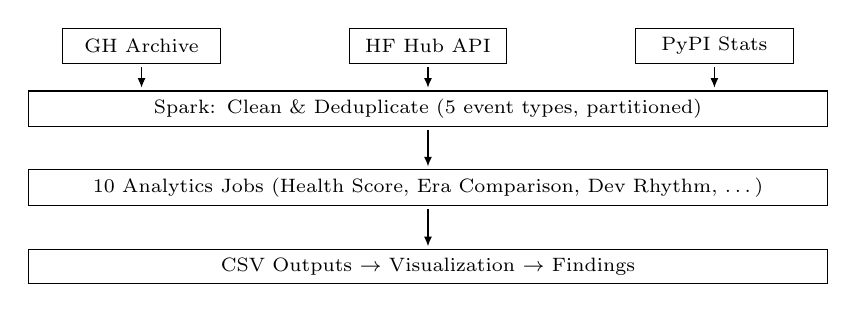
\begin{tikzpicture}[
  font=\scriptsize,
  src/.style    = {draw, rectangle, align=center, inner sep=2pt,
                   minimum height=4.5mm, minimum width=20mm},
  stage/.style  = {draw, rectangle, align=center, inner sep=3pt,
                   text width=0.82\columnwidth},
  arr/.style    = {-{Latex[length=1.2mm,width=1mm]},
                   shorten >=1pt, shorten <=1pt}
]
% Source row
\node[src] (gh) at (-0.30\columnwidth, 0) {GH Archive};
\node[src] (hf) at (0, 0)                  {HF Hub API};
\node[src] (py) at ( 0.30\columnwidth, 0) {PyPI Stats};

% Pipeline stages
\node[stage] (clean) at (0, -8mm)  {Spark: Clean \& Deduplicate (5 event types, partitioned)};
\node[stage] (jobs)  at (0, -18mm) {10 Analytics Jobs (Health Score, Era Comparison, Dev Rhythm, \ldots)};
\node[stage] (out)   at (0, -28mm) {CSV Outputs $\rightarrow$ Visualization $\rightarrow$ Findings};

% Arrows
\draw[arr] (gh.south) -- (gh.south  |- clean.north);
\draw[arr] (hf.south) -- (hf.south  |- clean.north);
\draw[arr] (py.south) -- (py.south  |- clean.north);
\draw[arr] (clean.south) -- (jobs.north);
\draw[arr] (jobs.south)  -- (out.north);
\end{tikzpicture}
\caption{Pipeline architecture: three data sources feed into Spark cleaning, then fan out to 10 analytics jobs.}\label{fig:pipeline}
\end{figure}

\subsection{Schema Design}

All five event types are mapped to a unified schema with 10 fields:
\texttt{event\_id}, \texttt{event\_type}, \texttt{event\_date} (partition key), \texttt{event\_ts}, \texttt{actor\_login}, \texttt{repo\_name}, \texttt{payload\_action}, \texttt{pr\_number}, \texttt{pr\_merged}, and \texttt{push\_distinct\_size}.

\subsection{Analytics Jobs}

Table~\ref{tab:jobs} summarizes the 10 analytics jobs.

\begin{table}[t]
\centering\scriptsize
\caption{Spark analytics jobs.}\label{tab:jobs}
\begin{tabular}{@{}clp{2.8cm}@{}}
\toprule
\textbf{\#} & \textbf{Output} & \textbf{Description} \\
\midrule
01 & repo\_daily          & Daily activity per AI repo \\
02 & hf\_gh\_join         & HF models + GH stats \\
03 & health\_score        & Composite health score \\
04 & top\_repos           & Top 1000 repos (ecosystem) \\
05 & ai\_vs\_general      & AI vs.\ general repos \\
06 & star\_hype           & Star growth \& hype \\
07 & contributor          & Bus factor, concentration \\
08 & era\_comparison      & Cross-era (5 Q1 snapshots) \\
09 & era\_deep\_dive      & Per-repo era analysis \\
10 & dev\_rhythm          & Weekend/weekday, push freq. \\
\bottomrule
\end{tabular}
\end{table}

% ══════════════════════════════════════════════════════════
\section{Data Quality}\label{sec:quality}

Across all five eras, the four core fields (\texttt{event\_type}, \texttt{event\_date}, \texttt{actor\_login}, \texttt{repo\_name}) have \textbf{zero nulls}.
Payload-specific fields (\texttt{pr\_merged}, \texttt{pr\_number}, \texttt{payload\_action}) are structurally null for non-applicable event types.

For the 2026-Q1 era, we re-downloaded all 2,160 raw hourly files and re-cleaned them.
580 corrupt gzip files were handled via Spark's \texttt{ignoreCorruptFiles} option.
Post-cleaning diff against the original was less than 0.39\%.
All eras are deduplicated by \texttt{event\_id}.

% ══════════════════════════════════════════════════════════
\section{Engineering Challenges}\label{sec:challenges}

\subsection{HDFS Quota Management}

Processing five years of Q1 data required ${\sim}$700~GB of raw storage, but the HDFS quota was 500~GB.

\textbf{Solution 1---Rolling pipeline:} Download one era's raw data, clean to Parquet, delete raw, proceed to next era. Storage stays under quota.

\textbf{Solution 2---Per-era processing:} Compute metrics for each era independently, save intermediate results. A final merge combines only small intermediate CSVs. If YARN terminates mid-job, completed eras are preserved.

\subsection{2026 Schema Breaking Change}

Job~08 initially reported zero merged PRs for 2026-Q1.
Investigation revealed that GitHub's REST/Webhook event payloads changed between 2025 and 2026~\cite{ghchangelog2025}: the \texttt{pr.merged} field became permanently \texttt{NULL}, replaced by a new \texttt{payload.action\,=\,"merged"} value, and the \texttt{push.distinct\_size} field was removed from \texttt{PushEvent} payloads (Table~\ref{tab:schema-change}). The latter prevents us from computing 1-commit-push ratios and average commit-size statistics for 2026-Q1.

\begin{table}[t]
\centering\small
\caption{GitHub API schema change.}\label{tab:schema-change}
\begin{tabular}{@{}lll@{}}
\toprule
\textbf{Field} & \textbf{$\leq$2025} & \textbf{2026+} \\
\midrule
\texttt{pr.merged}  & true/false & NULL \\
\texttt{action}     & open/close & + ``merged'' \\
\texttt{push.distinct\_size} & present & removed \\
\bottomrule
\end{tabular}
\end{table}

We implemented a backward-compatible fix:
\begin{lstlisting}[language=Python]
merged = (
  ((col("payload_action") == "closed")
   & col("pr_merged").eqNullSafe(True))
  | (col("payload_action") == "merged")
)
\end{lstlisting}

\subsection{Billion-Record Shuffle Optimization}

Computing top-1000 repos across 1B+ events required a full cross-partition shuffle (72~GB $\rightarrow$ 83~GB shuffle, $>$3 hours).
We tuned \texttt{shuffle.partitions} (400$\rightarrow$200), cached DataFrames, and downstream jobs read pre-aggregated outputs.
\textbf{Retrospective:} Bucketing by \texttt{repo\_name} at ingest would eliminate the shuffle entirely.

% ══════════════════════════════════════════════════════════
\section{Findings}\label{sec:findings}

\subsection{Finding 1: Five-Year Ecosystem Shift}

Figure~\ref{fig:era-shift} visualizes the ecosystem evolution; Table~\ref{tab:era-shift} presents the key metrics.

\begin{figure}[t]
\centering
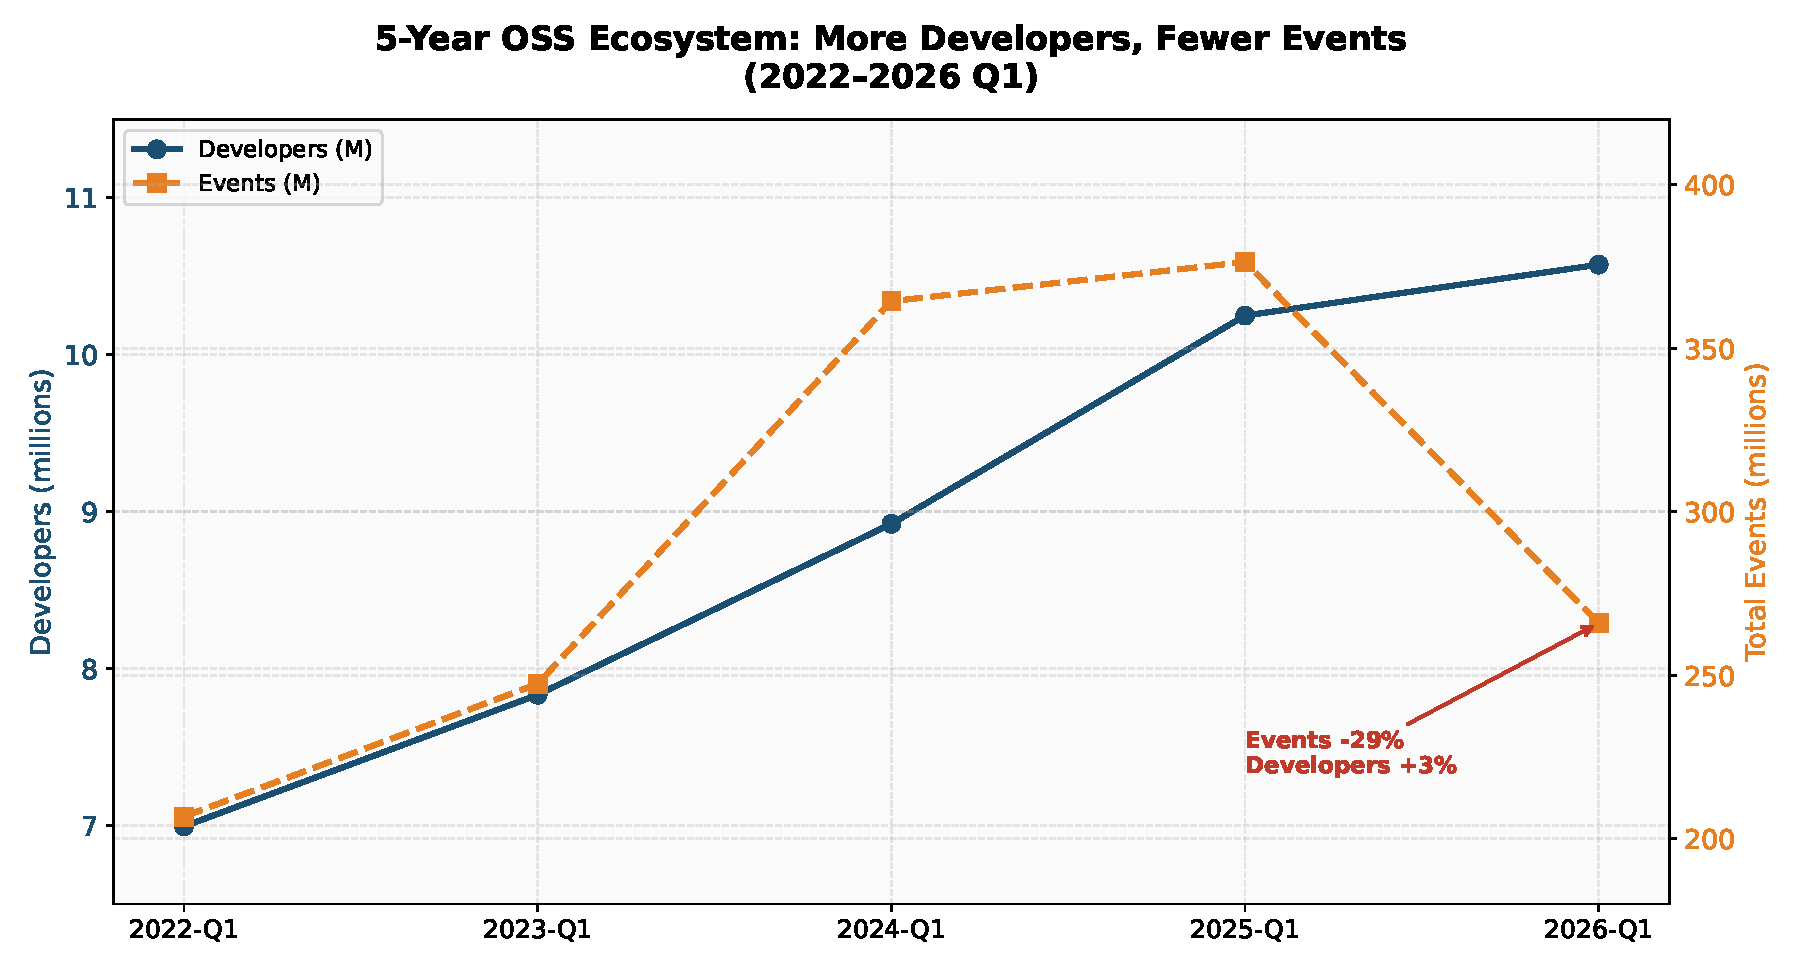
\includegraphics[width=\columnwidth]{03_era_shift.pdf}
\caption{Five-year ecosystem shift across 2022--2026 Q1 snapshots. Developers grew 51\% while contributors per repo fell 42\%.}\label{fig:era-shift}
\end{figure}

\begin{table}[t]
\centering\small
\caption{Ecosystem evolution: 2022 vs.\ 2026 Q1.
$^{\dagger}$1-commit push \% reports the latest era for which
\texttt{push.distinct\_size} is available (2025), since GitHub
removed this field in 2026 (\S\ref{sec:challenges}).}\label{tab:era-shift}
\begin{tabular}{@{}lrrr@{}}
\toprule
\textbf{Metric} & \textbf{2022} & \textbf{2026} & \textbf{$\Delta$} \\
\midrule
Developers        & 7.0M  & 10.6M & +51\% \\
Total events      & 207M  & 266M  & +29\% \\
1-commit push \%$^{\dagger}$ & 87\%  & 94\% (2025) & +7pp \\
PR/push ratio     & 0.098 & 0.082 & $-$16\% \\
Contrib./repo     & 4.88  & 2.84  & $-$42\% \\
\bottomrule
\end{tabular}
\end{table}

More developers are participating, but each repo receives fewer contributors.
Pushes are smaller and more frequent, while the PR/push ratio declined 16\%---less ceremony, more direct pushes.

\textbf{The 2026 event drop.}
Total events declined 29\% from 2025 to 2026.
The drop is concentrated in popularity signals (WatchEvents $-$63\%, ForkEvents $-$67\%) rather than in engineering activity (PushEvents $-$28\%).
\emph{PushEvent's share rose from 83\% in 2025 to 85\% in 2026 (versus 71\% in 2022).}
This pattern is consistent with the tail of GitHub's clean-up of suspected fake-star accounts reported by~\cite{he2024fakestars}, but several alternative or complementary explanations cannot be ruled out:
(i) the magnitude of the WatchEvent drop ($-$12.4M in a single quarter) exceeds what a one-time removal of $\sim$6M cumulative fake stars (2019--2024) can account for;
(ii) the 67\% ForkEvent decline is unlikely to be driven by fake-star clean-up, since forks are not the focus of that work;
(iii) the GitHub event-payload schema change of late 2025 (\S\ref{sec:challenges}) altered how some interactions are emitted; and
(iv) 580 corrupt hourly archives in 2026-Q1 were skipped via Spark's \texttt{ignoreCorruptFiles}, with an estimated cleaning-stage delta of $\le$0.39\% relative to a re-download (\S\ref{sec:quality}).
We therefore present this drop as an empirical observation rather than as evidence of any single cause.

\begin{figure}[t]
\centering
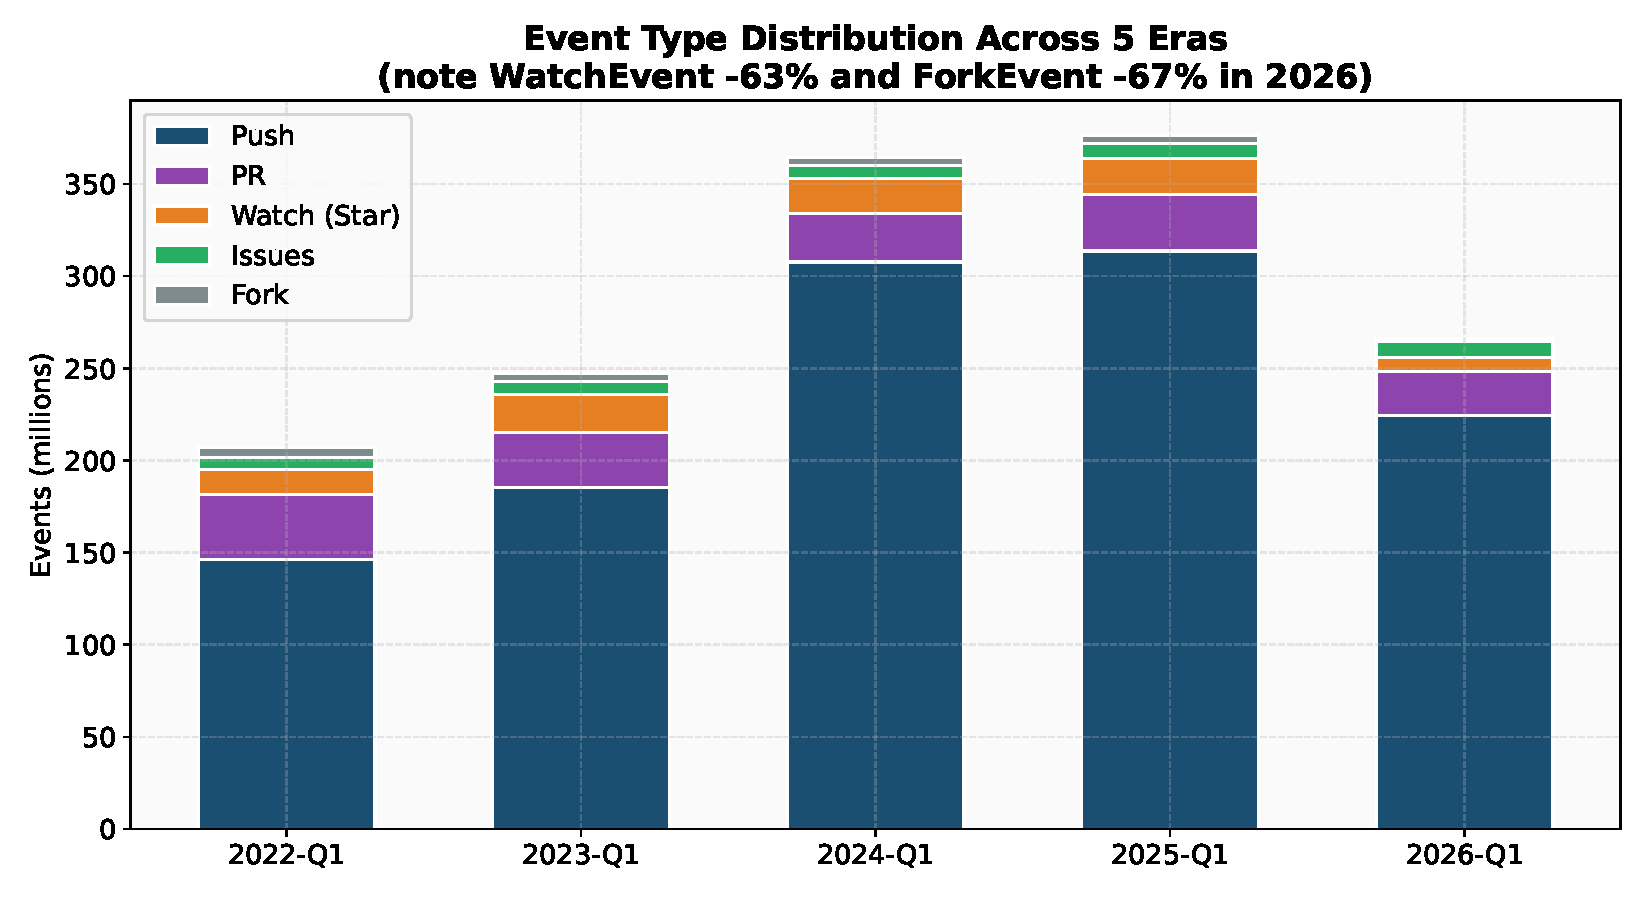
\includegraphics[width=\columnwidth]{07_event_distribution.pdf}
\caption{Event type composition across five eras. Push dominance grows as popularity signals (Watch, Fork) decline sharply in 2026.}\label{fig:event-dist}
\end{figure}

\subsection{Finding 2: The Weekend Gap Disappeared}

In a natural weekly distribution, weekends account for 28.9\% of days (2/7).
Human developers historically produce a weekend gap.
Figure~\ref{fig:weekend} shows this gap vanishing by 2026.

\begin{figure}[t]
\centering
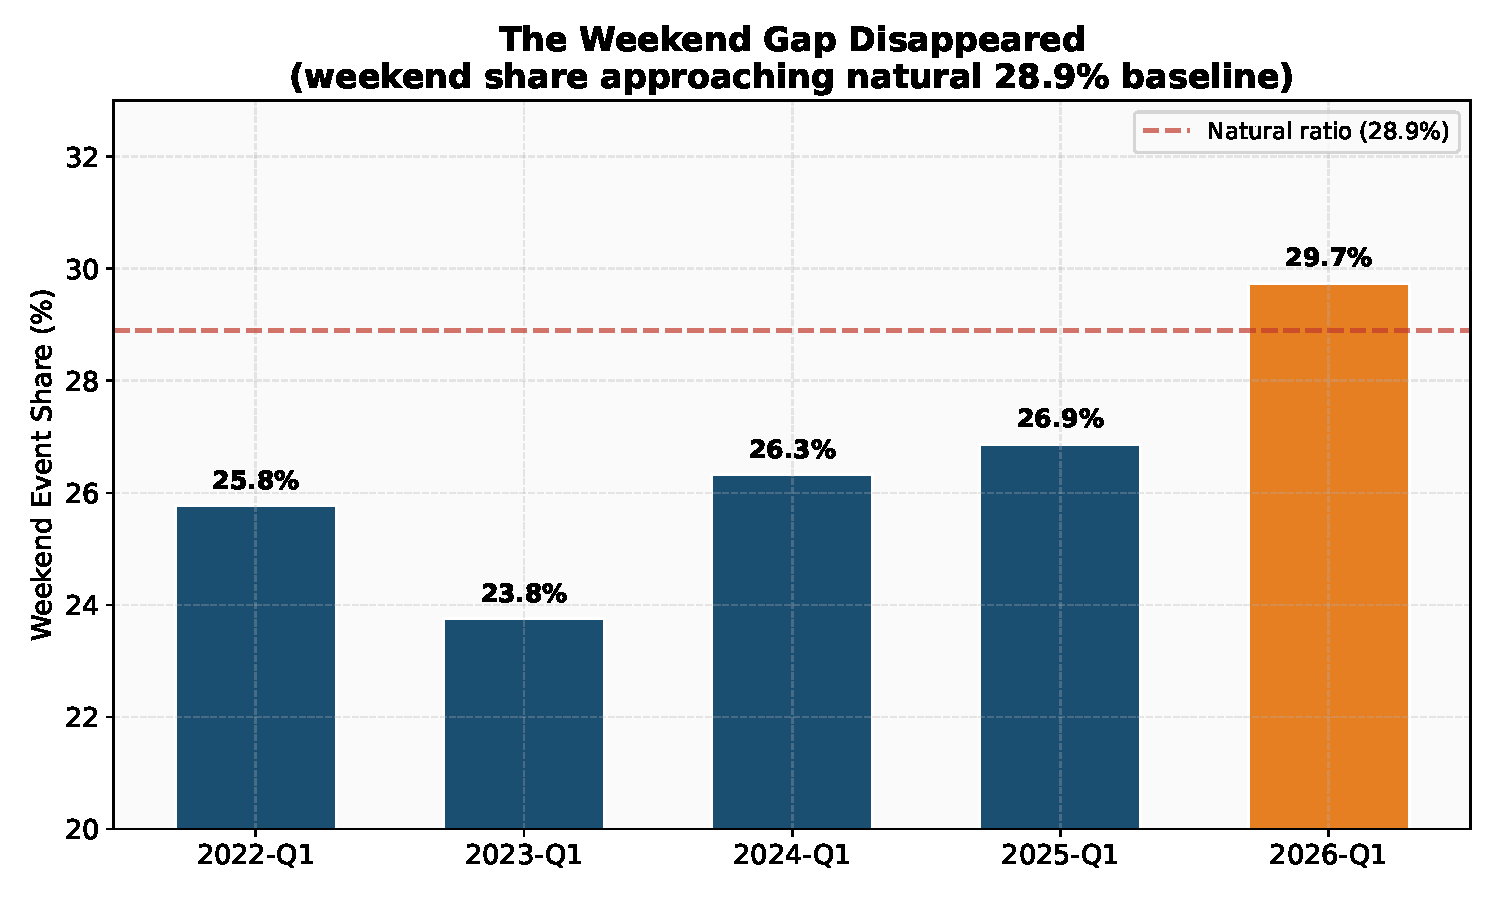
\includegraphics[width=\columnwidth]{04_weekend_gap.pdf}
\caption{Weekend event share across five eras. By 2026, weekend activity exceeds the 28.9\% natural baseline---a pattern compatible with round-the-clock automation, though human-side factors (globalization, on-call pressure) cannot be excluded.}\label{fig:weekend}
\end{figure}

\begin{table}[t]
\centering\small
\caption{Weekend event share across five eras.}\label{tab:weekend}
\begin{tabular}{@{}lcr@{}}
\toprule
\textbf{Era} & \textbf{Wknd \%} & \textbf{vs.\ 28.9\%} \\
\midrule
2022-Q1 & 25.8\% & $-$3.1pp \\
2023-Q1 & 23.7\% & $-$5.2pp \\
2024-Q1 & 26.3\% & $-$2.6pp \\
2025-Q1 & 26.9\% & $-$2.0pp \\
2026-Q1 & \textbf{29.7\%} & \textbf{+0.8pp} \\
\bottomrule
\end{tabular}
\end{table}

The closure is driven primarily by \texttt{PushEvent}, whose weekend ratio rose monotonically from 24.8\% (2022) to 29.4\% (2026). The \texttt{PullRequestEvent} weekend ratio is U-shaped over the same period (31.6\% $\rightarrow$ 18.4\% $\rightarrow$ 29.5\%), reflecting volatile bot-driven activity (Dependabot/Renovate \texttt{synchronize} events) rather than a uniform secular trend; we therefore anchor this finding on Push.
By 2026, push activity shows essentially no weekly periodicity. This is \emph{consistent with} (but not proof of) automated agents operating around the clock; alternative drivers---broader geographic participation, increased CI/CD automation, and weekend on-call work---would yield a similar signature and cannot be separated without actor-level labels.

\subsection{Finding 3: Two Phases of High-Frequency Push Activity}

We track \emph{high-frequency push accounts} ($>$1{,}000 pushes per quarter, or $>$50 pushes per day on the busiest day) as a proxy for automation-assisted activity. We caution that this cohort plausibly mixes coding agents, CI/build bots (e.g., the top pusher on \texttt{tensorflow/tensorflow} is a CI bot, see \S\ref{sec:stars}), scrapers, and a small number of human power users; the proxy therefore over-counts true agent adopters. With that caveat, the cohort exhibits a distinctive two-phase pattern (Figure~\ref{fig:agent-phases}, Table~\ref{tab:agent-phases}).

\begin{figure}[t]
\centering
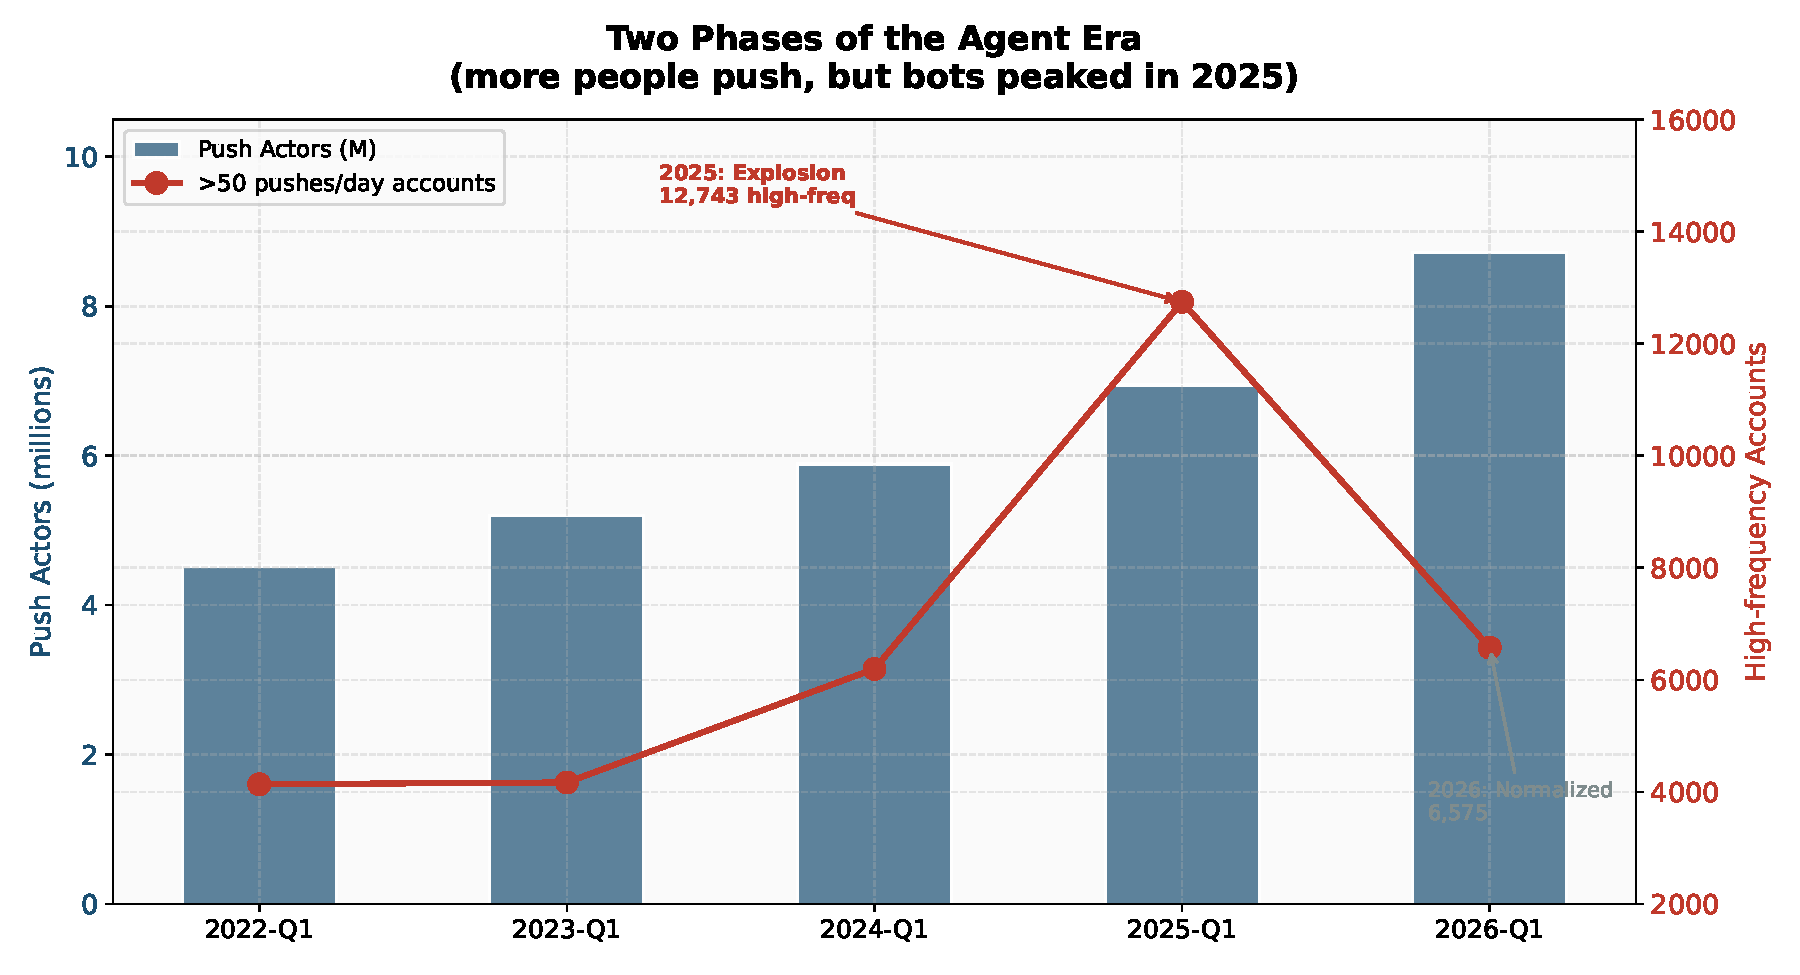
\includegraphics[width=\columnwidth]{05_agent_phases.pdf}
\caption{Two phases of high-frequency push activity: 2025 explosion (the $>$1K-pushes cohort nearly doubled) followed by 2026 normalization.}\label{fig:agent-phases}
\end{figure}

\begin{table}[t]
\centering\small
\caption{Push actor statistics (2024--2026).}\label{tab:agent-phases}
\begin{tabular}{@{}lrrr@{}}
\toprule
\textbf{Metric} & \textbf{'24} & \textbf{'25} & \textbf{'26} \\
\midrule
Push actors       & 5.89M & 6.95M & 8.71M \\
$>$1K pushes      & 5,347 & 9,788 & 6,351 \\
$>$50/day         & 6,197 & 12,743 & 6,575 \\
Avg push/actor    & 52.2  & 45.1  & 25.8 \\
Median pushes     & 6     & 6     & 4 \\
\bottomrule
\end{tabular}
\end{table}

\textbf{Phase 1---Explosion (2025):}
The $>$1K-pushes cohort nearly doubled (5{,}347$\rightarrow$9{,}788) and the $>$50-pushes-per-day cohort more than doubled. This is the kind of footprint expected from early automation adopters running coding agents and bots at superhuman rates, although individual-level confirmation is not possible from public event metadata alone.

\textbf{Phase 2---Normalization (2026):}
The high-frequency cohort dropped $-$35\%---a movement plausibly driven by GitHub's tightening of automation policies and bot clean-up---while total push actors grew to 8.71M (+25\%) and average pushes/actor fell 43\%.
The aggregate signature: \emph{more people push, but each pushes less.}

\subsection{Finding 4: Stars $\neq$ Health}\label{sec:stars}

Our composite health score reveals that star counts are weak predictors of project health:
\begin{align}\label{eq:health}
H = \;& 0.30\,S_{\text{HF}} + 0.20\,S_{\text{PyPI}} + 0.15\,S_{\star} \notag\\
      &+\; 0.15\,S_{\text{push}} + 0.10\,S_{\text{PR}} + 0.10\,S_{\text{days}}
\end{align}
where each $S$ is a min--max normalized score on the AI-repo subset.
Across the 33 AI repos with complete metadata, the Spearman rank correlation between GitHub stars and $H$ is only $\rho = 0.46$ (Pearson $r = 0.24$); only 4 of the top-10-by-stars repos appear in the top-10-by-$H$. Stars and downstream usage diverge substantially.

Figure~\ref{fig:stars-health} and Table~\ref{tab:archetypes} illustrate how three distinct archetypes emerge.

\begin{figure}[t]
\centering
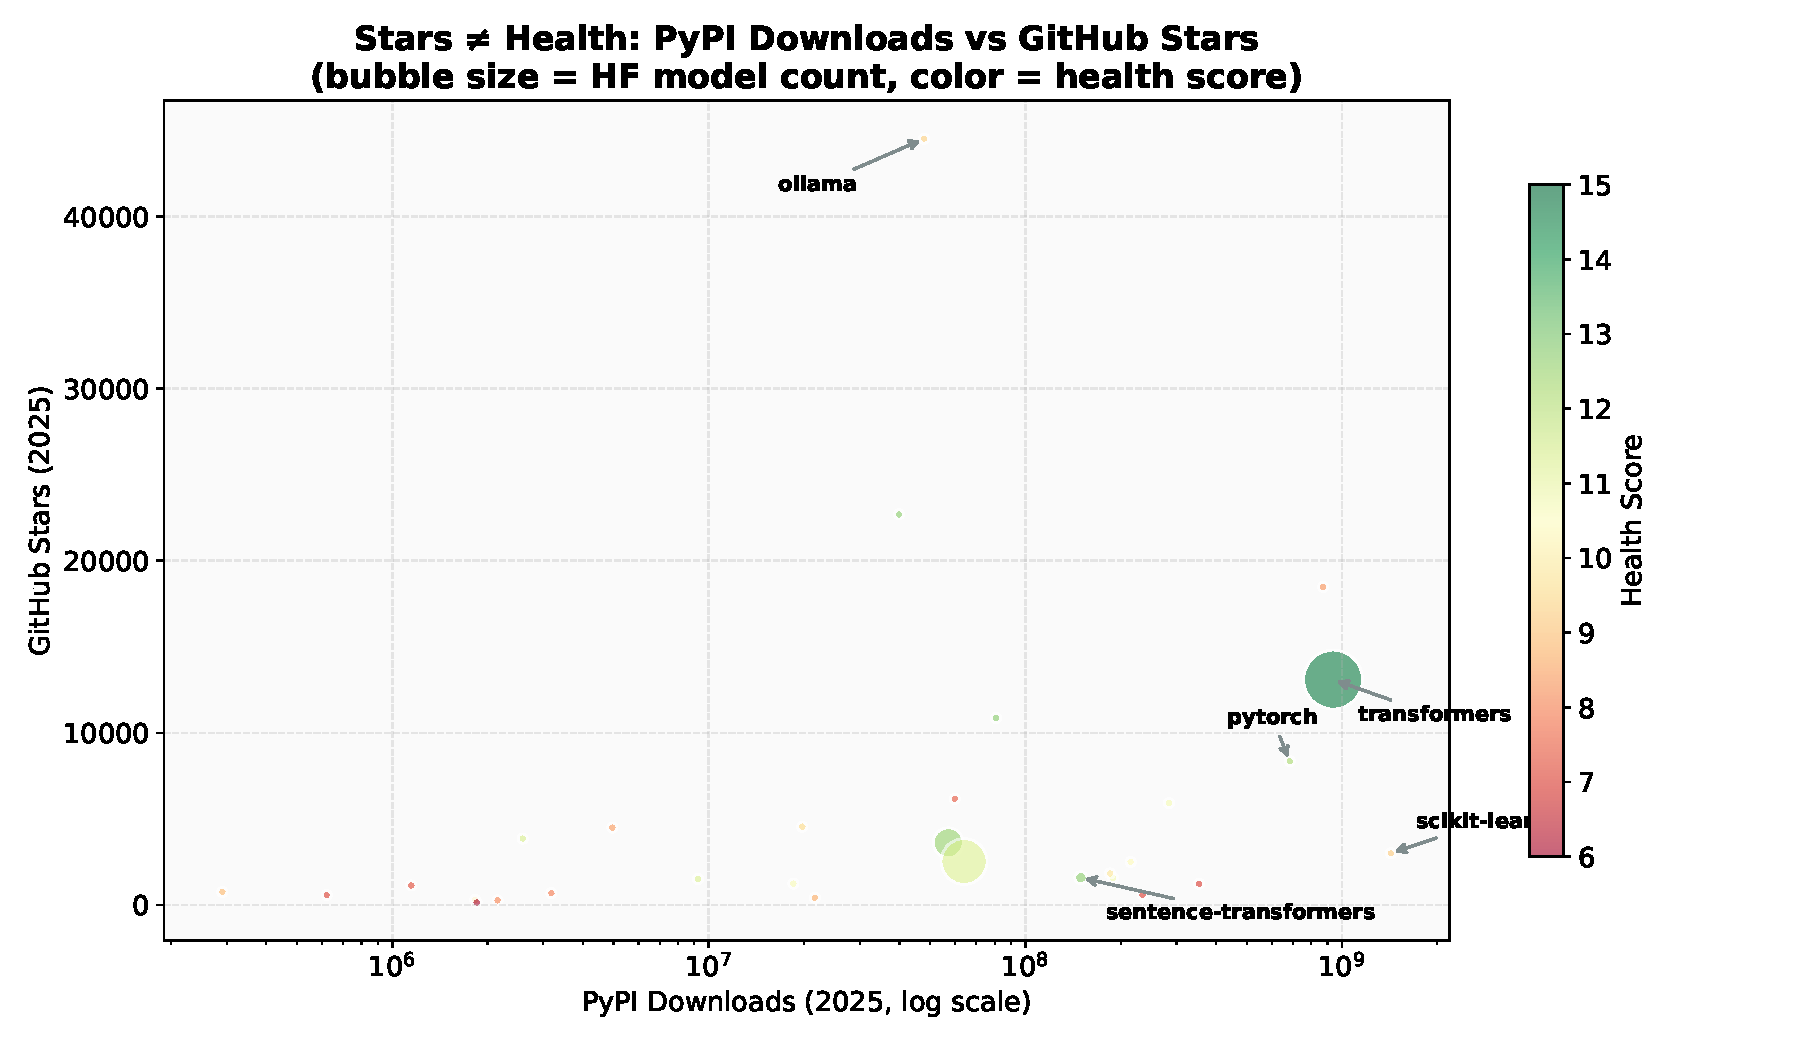
\includegraphics[width=\columnwidth]{01_stars_vs_health.pdf}
\caption{Stars vs.\ health score for AI repositories. High stars do not guarantee high health (e.g., Ollama).}\label{fig:stars-health}
\end{figure}

\begin{table}[t]
\centering\scriptsize
\setlength{\tabcolsep}{4pt}
\caption{Three health archetypes.}\label{tab:archetypes}
\begin{tabular}{@{}llrl@{}}
\toprule
\textbf{Archetype} & \textbf{Example} & \textbf{Stars} & \textbf{Usage Signal} \\
\midrule
True leader      & transformers & 13K   & PyPI 938M, HF 835K \\
Quiet power      & sent.-trans. & 1.6K  & HF 519M downloads \\
Eco.\ outsider   & ollama       & 44.5K & PyPI 47.8M, HF 241 \\
\bottomrule
\end{tabular}
\end{table}

Sentence-transformers has 1,588 stars but 519M HF downloads---invisible to star-based rankings.
Ollama has 44.5K stars but only 241 HF downloads, because it uses its own model registry.
No single metric suffices; triangulation is essential.

\subsection{Finding 5: Contributor Concentration}

AI repos exhibit systematically higher contributor concentration (Figure~\ref{fig:contributor-risk}).

\begin{figure}[t]
\centering
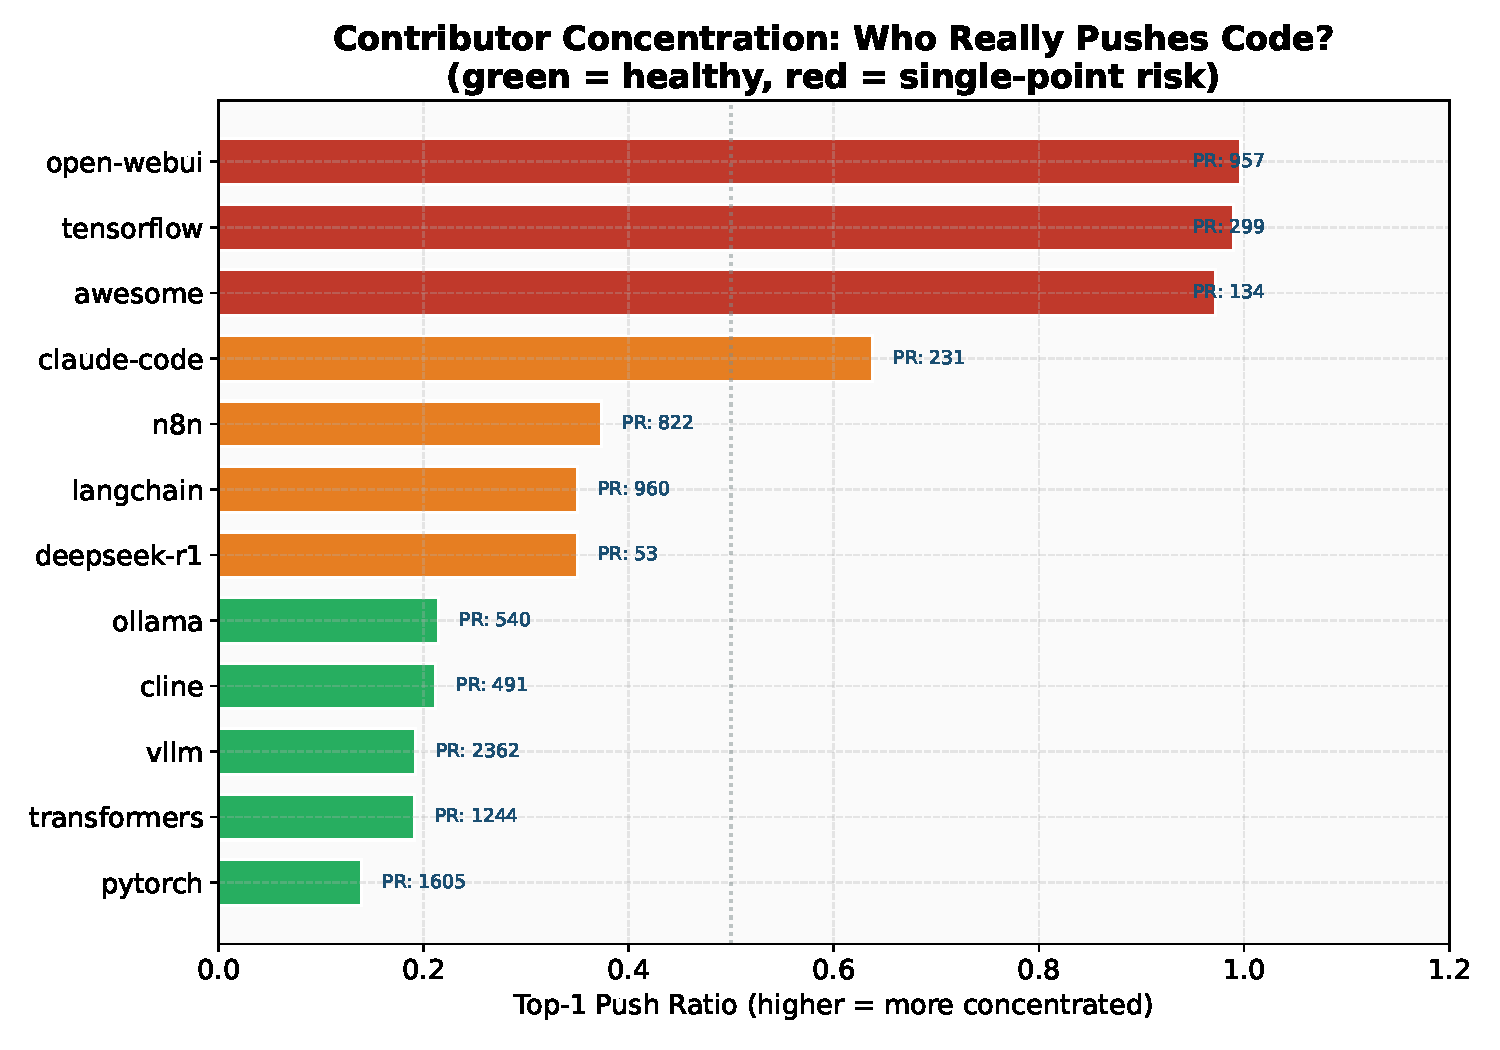
\includegraphics[width=\columnwidth]{02_contributor_risk.pdf}
\caption{Contributor concentration across top repositories. Red indicates high bus-factor risk.}\label{fig:contributor-risk}
\end{figure}

Key examples:
\begin{itemize}[nosep]
  \item \textbf{open-webui}: top1\_push\_ratio = 0.997 (one person, 99.7\% of pushes), yet 957 PR contributors.
  \item \textbf{DeepSeek-R1}: 93,947 watchers, 5 push contributors.
  \item \textbf{pytorch}: top1\_push\_ratio = 0.14, 1,605 PR contributors---healthy distribution.
\end{itemize}

As noted in \S\ref{sec:findings}, top pushers are sometimes CI bots (e.g., TensorFlow): push concentration must always be cross-validated with PR-author diversity before drawing bus-factor conclusions.

% ══════════════════════════════════════════════════════════
\section{Discussion}\label{sec:discussion}

\textbf{Implications for OSS health measurement.}
The ``GitHub stars'' metric is becoming actively misleading in the agent era.
As agents generate automated activity, the signal-to-noise ratio of any single metric degrades.
Multi-dimensional frameworks---combining community engagement (HF downloads), demand signals (PyPI installs), and engineering intensity (PRs, push diversity)---are necessary.

\textbf{The ``lighter development'' paradox.}
More developers than ever (10.6M, +51\%), yet per-repo contributor counts dropped 42\%.
One plausible reading is that automation lets individuals touch more projects simultaneously but with shallower per-project engagement; equally plausible is that the long tail of single-commit accounts grew without a matching growth in core maintainers. We cannot adjudicate between these from event-level data alone.

\textbf{24/7 development and sustainability.}
The vanished weekend gap raises sustainability questions, but it does not by itself indicate whether the additional weekend activity is automated or human.
Distinguishing human from automated event sources---through commit-message heuristics, signed-commit metadata, or actor-name patterns---is critical for future work.

\textbf{Limitations and threats to validity.}
\begin{itemize}[nosep]
  \item \emph{External:} Q1-only sampling may miss seasonal effects; the 93 seed repos may not represent the full AI ecosystem.
  \item \emph{Construct:} we cannot reliably distinguish agent-generated from human-generated events at the individual level, so ``high-frequency push activity'' is at best a proxy for agent adoption.
  \item \emph{Internal:} the 2026 event drop conflates the tail of GitHub's fake-star clean-up~\cite{he2024fakestars}, the late-2025 schema change~\cite{ghchangelog2025}, and possible genuine behavioral changes; we cannot decompose the contributions.
  \item \emph{Construct:} health-score weights are heuristic; a sensitivity analysis (e.g., equal weights or doubling $S_{\text{PyPI}}$) is left to future work but is not expected to overturn the qualitative ranking divergence reported in \S\ref{sec:stars}, given $\rho = 0.46$ between stars and $H$.
  \item \emph{Internal:} 580 corrupt 2026-Q1 hourly archives were skipped via \texttt{ignoreCorruptFiles}, contributing $\le$0.39\% to event counts.
\end{itemize}

% ══════════════════════════════════════════════════════════
\section{Lessons Learned}\label{sec:lessons}

\begin{enumerate}[nosep]
  \item \textbf{Design for the constraint.} The 500~GB quota forced a rolling pipeline that proved more crash-safe than a monolithic approach.
  \item \textbf{Never trust a live API schema.} The 2026 change silently broke our merge query---always assert assumptions.
  \item \textbf{Validate anomalies externally.} The 2026 event drop initially looked like a pipeline bug; cross-referencing the magnitude and timing with He et al.'s fake-star clean-up~\cite{he2024fakestars} and the 2025 GitHub event-payload schema change~\cite{ghchangelog2025} convinced us it reflected real, multi-cause platform-side effects rather than a defect in our pipeline.
\end{enumerate}

% ══════════════════════════════════════════════════════════
\section{Conclusion}\label{sec:conclusion}

We analyzed 1.46~billion GitHub events across the 2022--2026 coding-agent era, complemented by Hugging Face and PyPI data.
Five findings:

\begin{enumerate}[nosep]
  \item \textbf{Development got lighter}: +51\% developers, $-$42\% contributors per repo, smaller and more frequent pushes.
  \item \textbf{Weekends flattened}: Weekend activity reached 29.7\%, eliminating the historic human work--rest signal---compatible with, but not proof of, round-the-clock automation.
  \item \textbf{Two-phase high-frequency push activity}: 2025 explosion ($>$1K-pushes cohort nearly doubled) $\rightarrow$ 2026 normalization (broader but lighter), plausibly tracking but not equivalent to coding-agent adoption.
  \item \textbf{Stars $\neq$ health}: Spearman $\rho = 0.46$ between stars and our composite health score on the AI subset; only 4 of the top-10-by-stars repos appear in the top-10-by-$H$.
  \item \textbf{Concentrated authorship}: AI repos exhibit systematically higher push concentration; \texttt{open-webui} has one author responsible for 99.7\% of pushes despite 957 PR contributors. Push concentration must be cross-validated with PR-author diversity.
\end{enumerate}

Traditional metrics like stars are increasingly unreliable in isolation.
Multi-dimensional measurement---community adoption, package downloads, and engineering-activity diversity---is essential for accurate OSS health assessment.

\textbf{Future work} includes: developing actor-level heuristics to separate agent from human activity (commit message style, signing keys, naming patterns); extending to full-year coverage; incorporating code-review latency and issue-resolution time; sensitivity analysis on health-score weights; and longitudinal tracking of individual project health trajectories.

% ══════════════════════════════════════════════════════════
\section*{Acknowledgments}

We thank NYU High Performance Computing for providing the Google Cloud Dataproc cluster, GH Archive for open hourly event logs, Hugging Face Hub for public model metadata, and PyPI (via Google BigQuery) for download statistics.

\section*{Data and Code Availability}

The PySpark pipeline (10 analytics jobs), seed-repo list, and aggregated CSV outputs underlying every figure and table in this paper are organized in our project repository (\texttt{spark\_jobs/}, \texttt{data/}, \texttt{charts/}). All raw inputs are publicly redistributable from their original sources.

% ══════════════════════════════════════════════════════════
\bibliographystyle{plainnat}
\bibliography{references}

\end{document}
